%%%%%%%%%%%%%%%%%%%%%%%%%%%%%%%%%%%%%%%%%
% Medium Length Graduate Curriculum Vitae
% LaTeX Template
% Version 1.1 (9/12/12)
%
% This template has been downloaded from:
% http://www.LaTeXTemplates.com
%
% Original author:
% Rensselaer Polytechnic Institute (http://www.rpi.edu/dept/arc/training/latex/resumes/)
%
% Important note:
% This template requires the res.cls file to be in the same directory as the
% .tex file. The res.cls file provides the resume style used for structuring the
% document.
%
%%%%%%%%%%%%%%%%%%%%%%%%%%%%%%%%%%%%%%%%%

%----------------------------------------------------------------------------------------
%	PACKAGES AND OTHER DOCUMENT CONFIGURATIONS
%----------------------------------------------------------------------------------------

\documentclass[margin, 10pt]{res} % Use the res.cls style, the font size can be changed to 11pt or 12pt here
\usepackage{CJKutf8}
\usepackage{graphicx}
\usepackage{lipsum}
\usepackage{xcolor}
\usepackage{adjustbox}
\usepackage{helvet} % Default font is the helvetica postscript font
%\usepackage{newcent} % To change the default font to the new century schoolbook postscript font uncomment this line and comment the one above

\setlength{\textwidth}{5.1in} % Text width of the document

\begin{document}
%----------------------------------------------------------------------------------------
%	NAME AND ADDRESS SECTION
%----------------------------------------------------------------------------------------

\adjustbox{valign=t}{\begin{minipage}{0.20\linewidth}
\hspace*{-1.3in}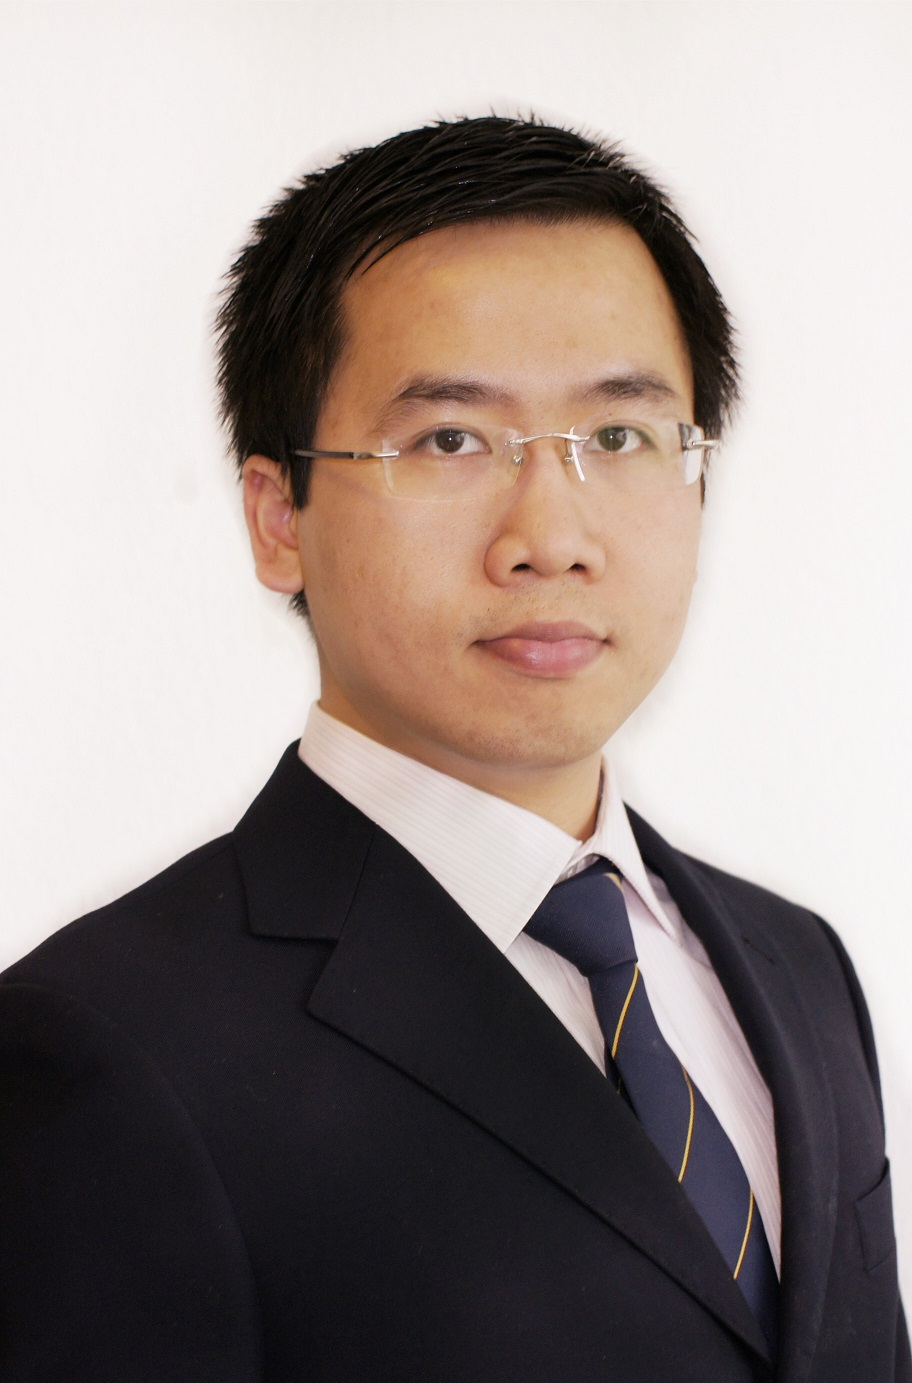
\includegraphics[width=1\linewidth]{photo.jpg}
\end{minipage}}%
\hfill
\adjustbox{valign=t}{\begin{minipage}[t]{0.77\linewidth}
\hspace*{-1.3in} \textbf{\fontsize{36}{36}\selectfont Jibin Ou} % Your name at the top
\newline
\hspace*{-1.3in} \vbox{\hrule width 1.3\textwidth height 1pt}\smallskip % Horizontal line after name; adjust line thickness by changing the '1pt'

\hspace*{-1.3in} \textbf{Nationality:} China, \textbf{Date of birth:} Sept. 1987 % Your address
\newline
\hspace*{-1.3in} \textbf{Current Address:} Jiading, Shanghai China
\newline
%\hspace*{-1.3in} \textbf{Home Address:} Sanshui District, Foshan City, Guangdong, China
%\newline
\hspace*{-1.3in} \textbf{E-Mail:} jibin.ou@outlook.com
\newline
\hspace*{-1.3in} \textbf{Website:} http://insyncim64.github.io
\newline
\hspace*{-1.3in} \textbf{Telephone:} +86-173-1762-6986
%\newline
%\hspace*{-1.3in} \textbf{Available from:} 01.10.2016
\newline
\hspace*{-1.3in} \textbf{Objective:} Core Java Software Engineer, Fullstack Software Engineer
\end{minipage}}

%----------------------------------------------------------------------------------------

\begin{resume}
\begin{CJK}{UTF8}{gbsn}

%----------------------------------------------------------------------------------------
%	OBJECTIVE SECTION
%----------------------------------------------------------------------------------------
 
%\section{OBJECTIVE}  

% A position in the field of internet and software industry in Europe with special interest in mobile application development

%----------------------------------------------------------------------------------------
%	EDUCATION SECTION
%----------------------------------------------------------------------------------------

\section{EDUCATION}
\textbf{M.Sc., media informatics} \hfill October 2010-April 2014 \\
RWTH Aachen, Aachen, Germany \\
\textbf{Visiting Student, computer science} \hfill July 2013-April 2014\\
ETH Zürich, Zürich, Switzerland   \\
\textbf{B.Sc, information and computational science} \hfill September 2006-June 2010\\
Sun Yat-sen University, Guangzhou, China
% \textbf{Visiting Student, mathematics} \hfill February 2009-June 2010  \\
% East China Normal University, Shanghai, China \\
 
%----------------------------------------------------------------------------------------
%	PROFESSIONAL EXPERIENCE SECTION
%----------------------------------------------------------------------------------------
 
\section{EXPERIENCE}

\textbf{Software Developer} \hfill October 2016–Current \\
Honeywell, Shanghai, Germany 

\begin{itemize} \itemsep -2pt % Reduce space between items
\item Be responsible for mobile client development for a global Internet of Things project in Honeywell;
\item Maintained local cloud instance for mainland China region;
\item Develop prove of concept IoT solutions for local customers;
\item Developed innovative projects and devoted ideas for new software solutions in logistics industry;
\end{itemize}

\textbf{Software Developer} \hfill January 2015–September 2016 \\
Honeywell, Mannheim, Germany 

\begin{itemize} \itemsep -2pt % Reduce space between items
\item Worked in client development team, responsible for the desktop client development that uses Java Swing and JavaFX framework for UI and sqlite database for data persistence;
\item Responsible for embedded device client which uses J2ME and Java Embedded framework, and is used for M2M communication;
\item Involved in client middleware development, which is used as the core component of different mobile clients;
\item Involved in backend development, that uses Spring framework for webservice development and Apache Cassandra for data persistence;
\end{itemize}

\textbf{Research Assistant} \hfill April 2014–December 2014 \\
Advanced Interactive Lab and Software Reliability Lab, ETH Zürich, Switzerland 

\begin{itemize} \itemsep -2pt % Reduce space between items
\item Researched state-of-the-art method for programming interface;
\item Responsible for developing generation visual programming tool using WPF framework as the front-end, and Eclipse RCP Plug-in as a back-end;
\item Co-authored SIG CHI conference paper;
\end{itemize}

\textbf{Development Intern} \hfill January 2013–June 2013 \\
Vehicle Integration and Validation Department, BMW Group, Munich, Germany 

\begin{itemize} \itemsep -2pt % Reduce space between items
\item Responsible for prototypes of a remote collaboration system, which facilitates the communication between different BMW plants globally.
\item Collaborated with colleagues from different departments to perform user study, collect user requirements and conducted the final user test.
\end{itemize}
 
\textbf{Research Assistant} \hfill July 2011-July 2012 \\
User-Centered Computing Group, Fraunhofer Institute for Applied Information Technology, Bonn, Germany
\begin{itemize}  \itemsep -2pt % Reduce space between items
\item Developed a real-time monitor and control service for home appliances, including a Android client, Java based back-end and Plugwise wireless power plugs.
\item Worked on using sensor fusion and ad-hoc Wi-Fi network to help generating more accurate location information.
\end{itemize} 

% \textbf{Intern} \hfill April 2009-August 2009\\
% Yves Rocher, Shanghai, China
% \begin{itemize} \itemsep -2pt % Reduce space between items
% \item Developed an online collaboration platform for the logistics team in Shanghai. 
% \item Maintained the server together with the technicians in the headquarter everyday.  
% \end{itemize} 

%----------------------------------------------------------------------------------------
%	COMPUTER SKILLS SECTION
%----------------------------------------------------------------------------------------
\section{COMPUTER \\ SKILLS}
\textbf{Language: }Java, C\#, Objective-C, JavaScript, Python, C\textbackslash C++\\
\textbf{Server-side: }SpringMVC, PostgreSQL, Apache Cassandra\\
\textbf{Browser-side: }Angular 2, Apache Cordova, TypeScript\\
\textbf{Client-side: }Swing\textbackslash AWT, iOS, Android, WPF\\
\textbf{Data analysis: }NumPy, TensorFlow\\
% \textbf{Hardware: }Microsoft Kinect, Raspberry Pi(GPIO)\\
\textbf{Tools: }Anaconda, LaTex, VBA\\
\textbf{Related course:} Machine Learning, Human Computer Interaction

%----------------------------------------------------------------------------------------
%	Project experience
%---------------------------------------------------------------------------------------- 

\section{SELECTED \\ PROJECTS}

\textbf{OBD based car diagnostic solution} \hfill October 2017-Current\\
Honeywell, Shanghai, China
\begin{itemize} \itemsep -2pt % Reduce space between items
	\item OBD based car diagnostic solution for second-hand car market;
	\item Be responsible for backend development, which is a Golang based RESTful API service and uses PostgreSQL and Apache Cassandra Database;
\end{itemize}

\textbf{Connected Freight solution} \hfill November 2016-August 2017\\
Honeywell, Shanghai, China
\begin{itemize} \itemsep -2pt % Reduce space between items
\item Developed client side and middleware which help user to monitor and interact with sensor gateway and tags;
\item Collaborated with teams in India, Germany and US to develop the solution;
\end{itemize}

\textbf{Mobile workflow management solution for Daimler} \hfill August 2015-March 2016\\
Honeywell, Mannheim, Germany
\begin{itemize} \itemsep -2pt % Reduce space between items
\item Responsible for development of a customized user login system, which works with the OPC communication system;
\item Collaborated in the test and deployment of the complete solution in work stations of factories;
\end{itemize}

%\textbf{Real estate transaction dashboard for Beijing, Shanghai and Guangzhou} \hfill January 2016-current\\
%Private project, Mannheim, Germany
%\begin{itemize} \itemsep -2pt % Reduce space between items
%\item Developed a website for query and visualization of sales information;
%\item Developed a Java based crawler to find information of first and second hand transaction information, a backend which uses SpringMVC and mongoDB, and a pure webapp frontend, which based on Angular 2, Bootstrap and TypeScript;
%\item Developing a work-in-progress extension is a Senenium-based crawler for crawling and saving articles from a WeChat public accounts;
%\end{itemize}

\textbf{Heap memory visualization and manipulation} \hfill July 2013-March 2014\\
ETH Zürich, Zürich, Switzerland
\begin{itemize} \itemsep -2pt % Reduce space between items
%\item Master thesis under supervision of Prof. Otmar Hilliges and Prof. Martin Vechev
\item Provided a basic mathematical model for visualizing and manipulating the objects and their relations in the heap;
\item Designed and developed a information visualization component using WPF and the heap traversal component using Eclipse RCP plug-in;
\end{itemize} 

% \textbf{WeAnnotate: A PDF viewer with notes sharing feature} \hfill Spring 2012\\
% RWTH Aachen, Aachen, Germany
% \begin{itemize} \itemsep -2pt % Reduce space between items
% \item Acted as a team leader in the semester project of course {\sl Advanced Learning Technology };
% \item Built an Android tablet client application with MuPDF framework to display PDF files, and a back-end based on Google App Engine.
% \end{itemize}

%\textbf{Location-based pong game} \hfill Spring 2012\\
%Fraunhofer FIT, Bonn, Germany
%\begin{itemize} \itemsep -2pt % Reduce space between items
%\item {Built the network layer to achieve P2P communication via WiFi using Qualcomm Alljoyn framework.}
%\item {Examined different kinds of technologies including GPS, WiFi finger printing, WiFi signal strength and motion sensors to locate the user's position.}
%\end{itemize}$

%\textbf{ShadowBall: A mixed-reality game based on Microsoft Kinect sensor} \hfill Spring 2011\\
%Fraunhofer FIT, Bonn, Germany
%\begin{itemize} \itemsep -2pt % Reduce space between items
%\item {A mixed-reality game which uses Microsoft Kinect sensor and allows players to use their body parts to interact with the on-screen elements.}
%\item {Conducted user studies; Retrieved, analysed and manipulated the depth map using openNI and openCV.}
%\end{itemize}

%----------------------------------------------------------------------------------------
%	Publication
%----------------------------------------------------------------------------------------
\section{PUBLICATION} 
Jibin Ou, Martin Vechev, Otmar Hilliges. \textbf{An Interactive System for Data Structure Development}.
In Proc. Computer Human Interaction(CHI) 2015, Seoul Korea.(average acceptance rate 20\%)

%----------------------------------------------------------------------------------------
%	COMPUTER SKILLS SECTION
%----------------------------------------------------------------------------------------

\section{LANGUAGE}
English(professional proficiency), German(advanced), Chinese(mother tongue), Cantonese(mother tongue)

%----------------------------------------------------------------------------------------
%	EXTRA-CURRICULAR ACTIVITIES SECTION
%----------------------------------------------------------------------------------------

\section{EXTRA-CURRICULAR \\ ACTIVITIES} 
Won {\it Bravo Gold Recognition}, Honeywell, Shanghai, November 2016 and July 2017 \\
Won {\it IDEA League Student Research Scholarship}, IDEA League, Zürich, 2013 \\
% Won {\it Exceptional Outstanding Student Scholarship}, Sun Yat-sen University, Guangzhou, both 2007 and 2008 \\

%----------------------------------------------------------------------------------------
\end{CJK}
\end{resume}
\end{document}